% ============================================================
%  6.5 Metodología CRISP-DM   (capítulo 6, Marco teórico)
%  Se incluye desde secciones/07_marco_teorico.tex con \input.
% ============================================================
\section{Metodología CRISP-DM}
\label{sec:crisp-dm}

CRISP-DM (\textit{Cross-Industry Standard Process for Data Mining}) es un modelo de proceso
para proyectos de minería de datos, desarrollado a finales de la década de 1990 por un
consorcio de empresas en el marco de un proyecto financiado por la Unión Europea y publicado
como guía de referencia en su versión~1.0 \parencite{chapman2000}. Su propósito es ofrecer
un marco independiente de la industria, de la herramienta y de la aplicación, que haga los
proyectos más fiables, repetibles, manejables y menos costosos \parencite{wirth2000}. El
modelo organiza el ciclo de vida del proyecto en seis fases: comprensión del negocio, en la
que se definen los objetivos y requisitos desde la perspectiva de la organización y se
traducen en un problema analítico; comprensión de los datos, que comprende la recolección
inicial, la descripción, la exploración y la verificación de la calidad; preparación de los
datos, que abarca la selección, limpieza, construcción, integración y formateo del conjunto
de datos final; modelado, en el que se seleccionan y aplican las técnicas y se calibran sus
parámetros; evaluación, en la que se valora si los modelos satisfacen los objetivos del
negocio y se revisa el proceso; y despliegue, en el que el conocimiento obtenido se organiza
y presenta de forma que la organización pueda utilizarlo, incluyendo la planificación del
monitoreo y el mantenimiento \parencite{chapman2000}.

\begin{figure}[H]
  \centering
  \caption{Fases de la metodología CRISP-DM}
  \label{fig:crisp-dm}
  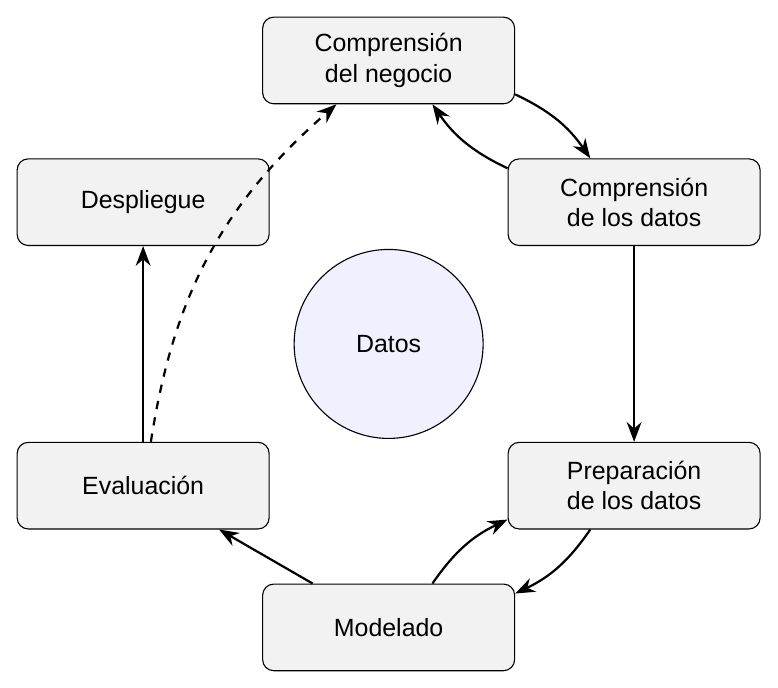
\includegraphics[width=0.6\textwidth]{imagenes/06_marco_teorico/crisp_dm.png}
  \fuente{Adaptado de \textcite{chapman2000}.}
\end{figure}

Una característica central de CRISP-DM es su carácter iterativo: la secuencia de fases no es
rígida, y el modelo contempla de forma explícita el retorno a fases anteriores cuando los
hallazgos lo requieren, por ejemplo cuando la exploración de los datos obliga a reformular
el objetivo o cuando el modelado revela la necesidad de nuevas variables. El ciclo externo
del diagrama de referencia (figura~\ref{fig:crisp-dm}) expresa, además, que el propio proceso
de minería de datos continúa tras el despliegue, porque las lecciones aprendidas generan
nuevas preguntas. La guía de referencia reconoce también que la preparación de los datos
suele concentrar la mayor parte del esfuerzo de un proyecto, un rasgo que se acentúa en
proyectos geoespaciales que integran fuentes heterogéneas.

CRISP-DM no es el único marco disponible. El proceso de descubrimiento de conocimiento en
bases de datos (KDD), descrito por \textcite{fayyad1996}, organiza el trabajo en etapas de
selección, preprocesamiento, transformación, minería de datos e interpretación o evaluación,
con un énfasis mayor en el proceso técnico de extracción de patrones que en la comprensión
del negocio. SEMMA, propuesto por SAS Institute, estructura el trabajo en las etapas de
muestreo, exploración, modificación, modelado y evaluación (\textit{Sample, Explore, Modify,
Model, Assess}), y está estrechamente asociado a las herramientas de ese proveedor. Frente a
ambos, CRISP-DM se distingue por incorporar explícitamente la comprensión del negocio y el
despliegue. En años recientes se han propuesto extensiones: \textcite{martinez2021}
analizaron la vigencia de CRISP-DM veinte años después de su creación y propusieron un marco
de trayectorias de ciencia de datos que reconoce que los proyectos actuales no siempre
siguen un ciclo lineal orientado a un modelo, sino recorridos exploratorios diversos; y
\textcite{studer2021} formularon CRISP-ML(Q), un modelo de proceso para aplicaciones de
aprendizaje automático con una metodología de aseguramiento de la calidad, que abarca seis
fases desde la definición del alcance hasta el mantenimiento de la aplicación desplegada,
ejecuta simultáneamente la comprensión del negocio y la de los datos, e incorpora de forma
explícita el monitoreo y el mantenimiento del modelo en operación frente a riesgos como la
deriva de los datos.

Se adopta CRISP-DM en este proyecto por su amplia aceptación en la práctica y en la
formación académica, por su énfasis en la comprensión del problema de la organización
destinataria y por su compatibilidad con las extensiones de CRISP-ML(Q) para la fase de
despliegue. Conforme a esta metodología, el proyecto se estructura de la siguiente manera.
En la comprensión del negocio se define el problema de los voluntarios de la Trufi
Association, que consiste en priorizar dónde revisar o mapear rutas, y se traduce en el
estimando del proyecto: el número esperado de consultas de cada zona dada su población y su
contexto territorial, cuyo contraste con lo observado orienta la priorización. En la
comprensión de los datos se exploran las consultas semanales y su distribución espacial y
temporal, se caracteriza el período sin datos de siete semanas, se examinan las ediciones de
población de Kontur y el feed GTFS de Trufi, y se analiza la autocorrelación espacial de las
consultas. En la preparación de los datos se depuran las consultas, se asignan a zonas H3 de
resolución~8, se integran con la población y con la cobertura medida como distancia al
trazado, y se construyen las macrozonas de resolución~6 que sirven como bloques de
validación. En el modelado se compara la escalera de técnicas descrita en
\ref{sec:tecnicas-algoritmos} mediante validación cruzada espacial por bloques. En la
evaluación se aplica una única vez el conjunto de prueba reservado, se calculan las métricas
descritas en \ref{sec:metricas}, se aplica la regla de selección declarada de antemano y se
realizan los análisis de sensibilidad y de estabilidad de la priorización. Finalmente, el
despliegue se limita a una propuesta de pipeline reproducible de actualización, que permita
reejecutar el proceso con nuevas consultas y nuevas ediciones de población y monitorear la
deriva de los datos al estilo de CRISP-ML(Q), junto con los entregables del proyecto, que
son un mapa interactivo, un archivo de estimaciones por zona y una lista de zonas
prioritarias para revisión, sin implementación operativa en los sistemas de Trufi.
